% Thesis print version of flow_oliver_solution_loop (19 Oct 2026): 12 pt base and every font one step larger,
% so the text prints at 7.5 pt or more at text width. Build: pdflatex flow_oliver_solution_loop_print.tex
\documentclass[tikz,border=3pt,12pt]{standalone}
\usepackage{amsmath,amssymb}
\usepackage{mathptmx}
\usepackage{bm}
\usepackage{tikz}
\usetikzlibrary{shapes.geometric,arrows.meta,positioning,fit,backgrounds,calc}
\let\origsmall\small \let\orignormalsize\normalsize \let\origfootnotesize\footnotesize
\renewcommand{\scriptsize}{\origfootnotesize}
\renewcommand{\footnotesize}{\origsmall}
\renewcommand{\small}{\orignormalsize}
\newcommand{\olboxwidth}{11cm}
\begin{document}
\providecommand{\olboxwidth}{9.6cm}% main box width (the thesis print version sets 11cm)
% flow_oliver_solution_loop.tex — the solution loop of the partner ANSYS/UPF
% framework, and where our constitutive law attaches to it.
%
% Traced from the source pool (USolBeg / Usermat / USSFin), as recorded in
% ansys_usermat/OLIVER_MODEL_NOTES.md §"How the whole thing runs". Everything
% in solid boxes is read directly from the code; the one interpretation is
% marked as such. Usage:
%   \resizebox{\linewidth}{!}{\providecommand{\olboxwidth}{9.6cm}% main box width (the thesis print version sets 11cm)
% flow_oliver_solution_loop.tex — the solution loop of the partner ANSYS/UPF
% framework, and where our constitutive law attaches to it.
%
% Traced from the source pool (USolBeg / Usermat / USSFin), as recorded in
% ansys_usermat/OLIVER_MODEL_NOTES.md §"How the whole thing runs". Everything
% in solid boxes is read directly from the code; the one interpretation is
% marked as such. Usage:
%   \resizebox{\linewidth}{!}{\providecommand{\olboxwidth}{9.6cm}% main box width (the thesis print version sets 11cm)
% flow_oliver_solution_loop.tex — the solution loop of the partner ANSYS/UPF
% framework, and where our constitutive law attaches to it.
%
% Traced from the source pool (USolBeg / Usermat / USSFin), as recorded in
% ansys_usermat/OLIVER_MODEL_NOTES.md §"How the whole thing runs". Everything
% in solid boxes is read directly from the code; the one interpretation is
% marked as such. Usage:
%   \resizebox{\linewidth}{!}{\input{flow_oliver_solution_loop.tex}}
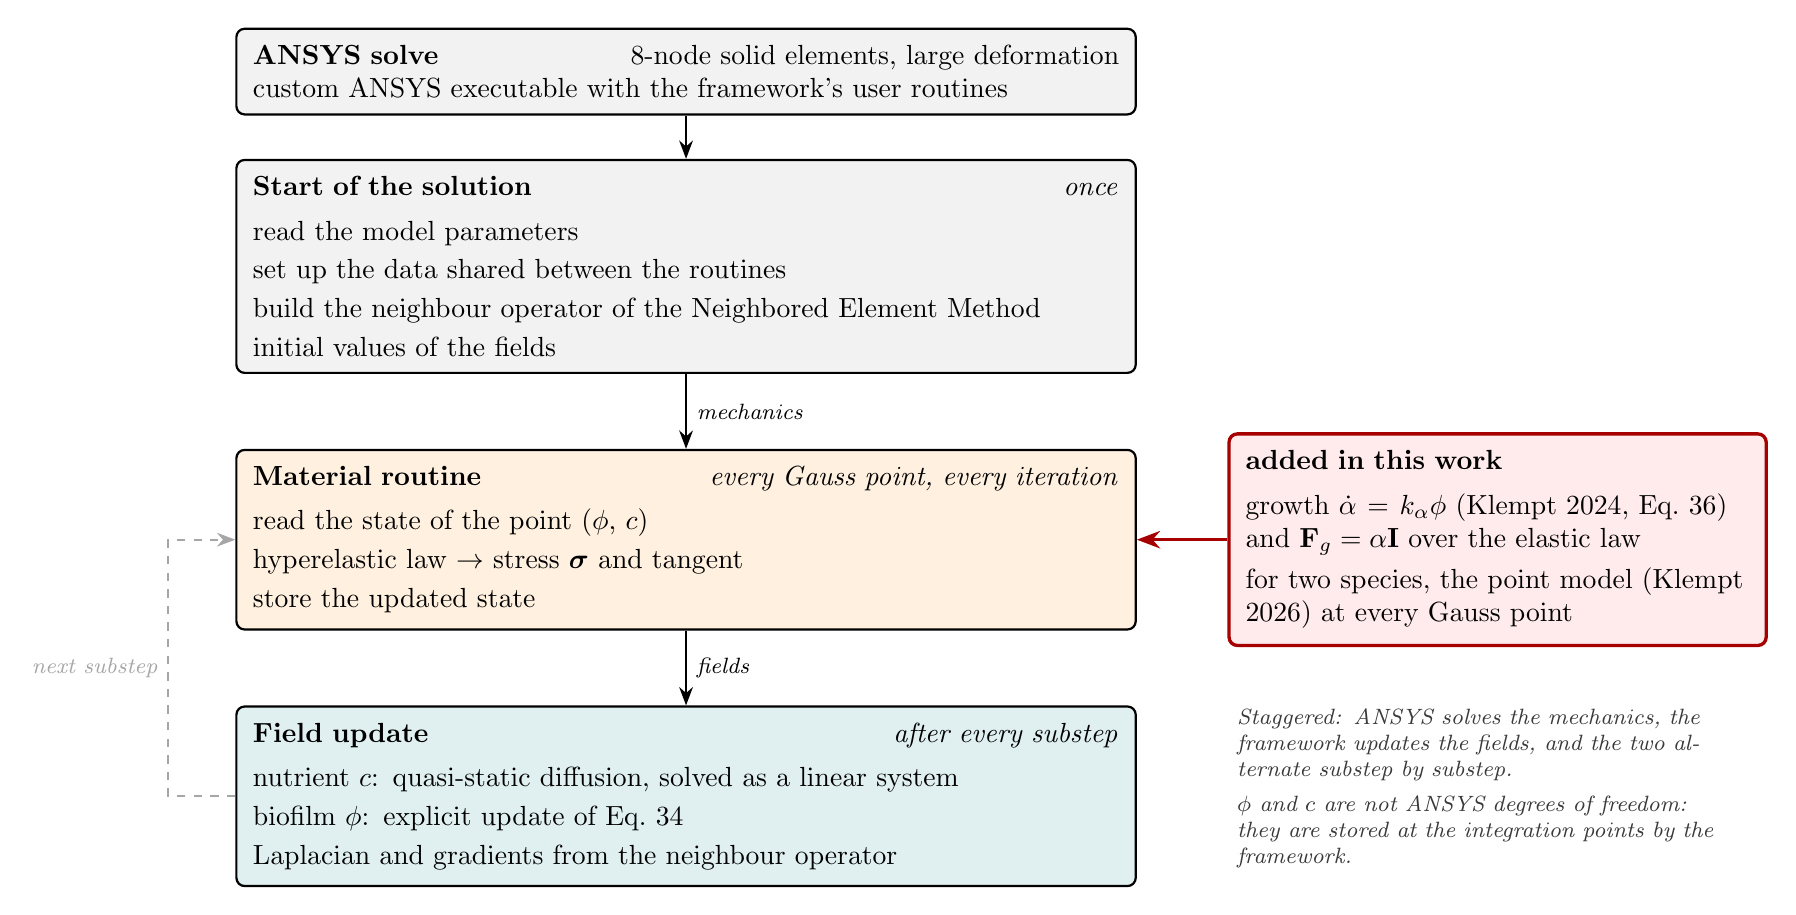
\begin{tikzpicture}[
  every node/.style = {font=\small},
  N/.style    = {draw, rounded corners=3pt, align=left, thick,
                 text width=\olboxwidth, inner sep=6pt},
  Nonce/.style= {N, fill=gray!10},
  Ngp/.style  = {N, fill=orange!12},
  Nfld/.style = {N, fill=teal!12},
  Nours/.style= {draw, rounded corners=3pt, align=left, very thick,
                 draw=red!65!black, fill=red!8, text width=6.4cm, inner sep=6pt},
  ar/.style   = {-Stealth, thick},
  arb/.style  = {-Stealth, thick, dashed, gray!70},
  lbl/.style  = {font=\scriptsize\itshape, fill=white, inner sep=1.5pt, align=center},
  note/.style = {font=\scriptsize\itshape, align=left, text width=6.2cm, gray!45!black},
]

% ── entry ───────────────────────────────────────────────────────────
% Reworded 6 Oct 2026 for the thesis: what each stage does, without the
% framework's internal routine and variable names and without the inherited
% lines that play no part in this work.
\node[Nonce] (top) {%
  \textbf{ANSYS solve} \hfill 8-node solid elements, large deformation\\
  custom ANSYS executable with the framework's user routines};

% ── start of the solution ──────────────────────────────────────────
\node[Nonce, below=0.55cm of top] (beg) {%
  \textbf{Start of the solution} \hfill \textit{once}\\[4pt]
  read the model parameters\\[2pt]
  set up the data shared between the routines\\[2pt]
  build the neighbour operator of the Neighbored Element Method\\[2pt]
  initial values of the fields};
\draw[ar] (top) -- (beg);

% ── the staggered loop ──────────────────────────────────────────────
\node[Ngp, below=0.95cm of beg] (gp) {%
  \textbf{Material routine} \hfill \textit{every Gauss point, every iteration}\\[4pt]
  read the state of the point ($\phi$, $c$)\\[2pt]
  hyperelastic law $\rightarrow$ stress $\bm\sigma$ and tangent\\[2pt]
  store the updated state};
\draw[ar] (beg) -- node[lbl,right,xshift=2pt] {mechanics} (gp);

\node[Nfld, below=0.95cm of gp] (fld) {%
  \textbf{Field update} \hfill \textit{after every substep}\\[4pt]
  nutrient $c$: quasi-static diffusion, solved as a linear system\\[2pt]
  biofilm $\phi$: explicit update of Eq.~34\\[2pt]
  Laplacian and gradients from the neighbour operator};
\draw[ar] (gp) -- node[lbl,right,xshift=2pt] {fields} (fld);

% staggered feedback
\draw[arb] (fld.west) -- ++(-0.85,0) |- node[lbl,pos=0.25,left,xshift=-2pt]
  {next substep} (gp.west);

% ── attachment point of this work ───────────────────────────────────
\node[Nours, right=1.15cm of gp] (ours) {%
  \textbf{added in this work}\\[4pt]
  \small growth $\dot\alpha=k_\alpha\phi$ (Klempt 2024, Eq.~36) and
  $\mathbf F_g=\alpha\mathbf I$ over the elastic law\\[3pt]
  \small for two species, the point model (Klempt 2026) at every Gauss point};
\draw[ar, draw=red!65!black, very thick] (ours) -- (gp);

% ── annotation ──────────────────────────────────────────────────────
\node[note, right=1.15cm of fld, yshift=0.1cm] (n1) {%
  Staggered: ANSYS solves the mechanics, the framework updates the fields,
  and the two alternate substep by substep.\\[3pt]
  $\phi$ and $c$ are not ANSYS degrees of freedom: they are stored at the
  integration points by the framework.};

\end{tikzpicture}
}
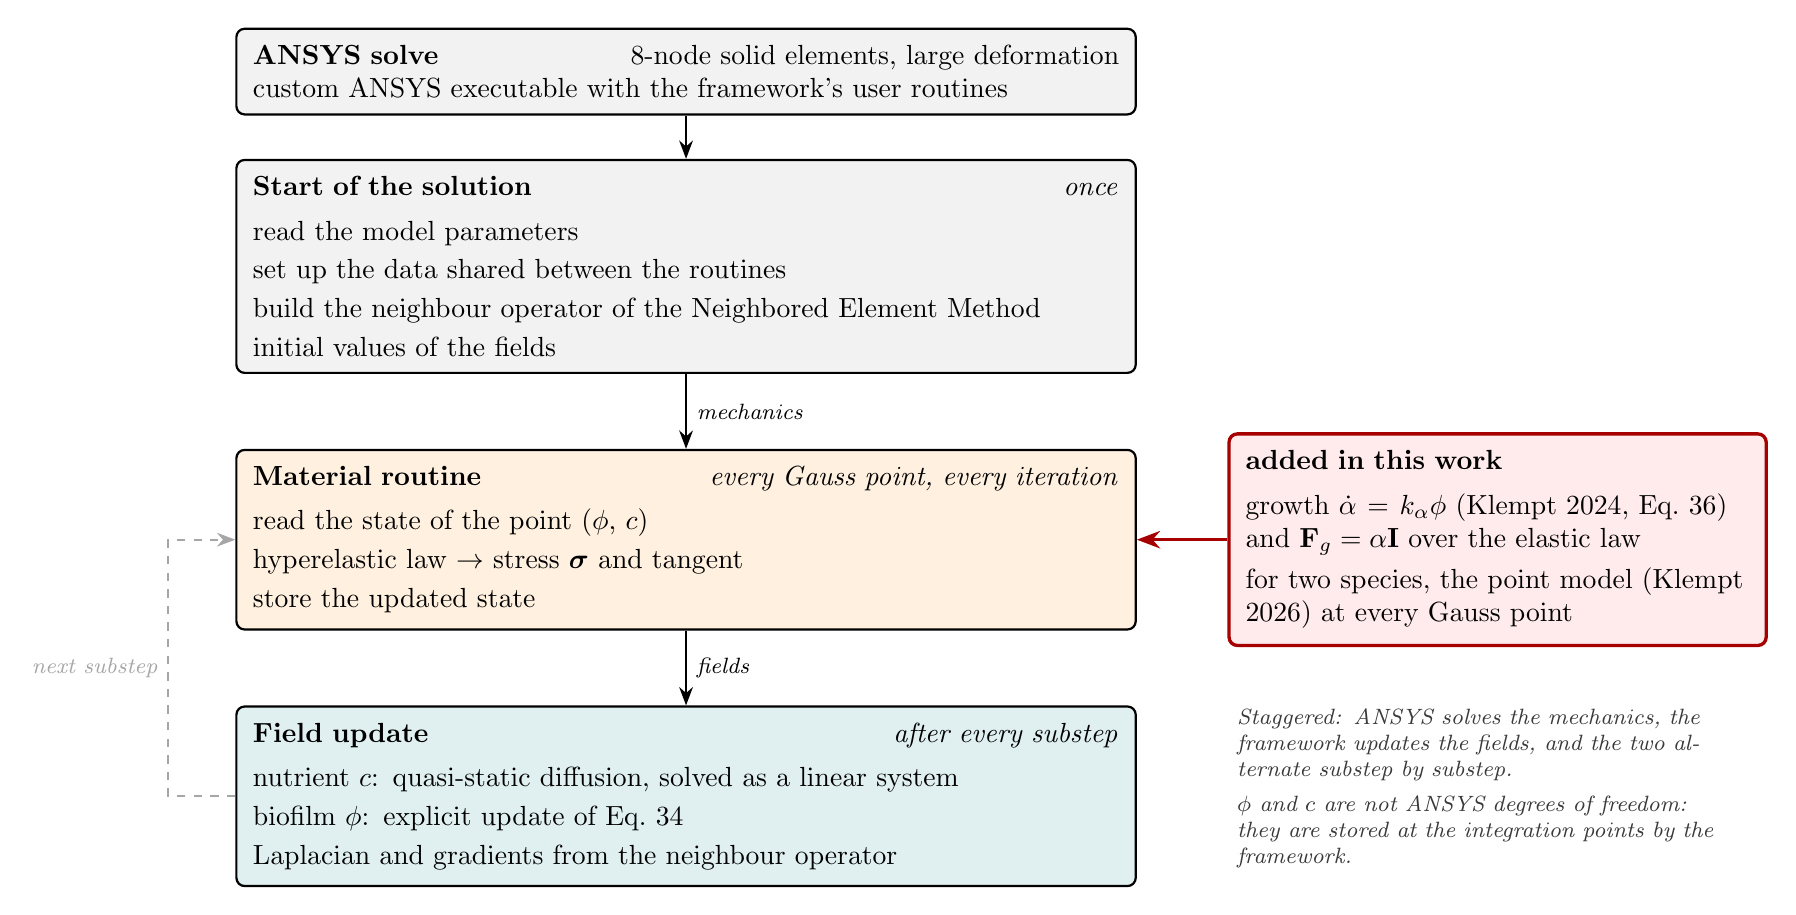
\begin{tikzpicture}[
  every node/.style = {font=\small},
  N/.style    = {draw, rounded corners=3pt, align=left, thick,
                 text width=\olboxwidth, inner sep=6pt},
  Nonce/.style= {N, fill=gray!10},
  Ngp/.style  = {N, fill=orange!12},
  Nfld/.style = {N, fill=teal!12},
  Nours/.style= {draw, rounded corners=3pt, align=left, very thick,
                 draw=red!65!black, fill=red!8, text width=6.4cm, inner sep=6pt},
  ar/.style   = {-Stealth, thick},
  arb/.style  = {-Stealth, thick, dashed, gray!70},
  lbl/.style  = {font=\scriptsize\itshape, fill=white, inner sep=1.5pt, align=center},
  note/.style = {font=\scriptsize\itshape, align=left, text width=6.2cm, gray!45!black},
]

% ── entry ───────────────────────────────────────────────────────────
% Reworded 6 Oct 2026 for the thesis: what each stage does, without the
% framework's internal routine and variable names and without the inherited
% lines that play no part in this work.
\node[Nonce] (top) {%
  \textbf{ANSYS solve} \hfill 8-node solid elements, large deformation\\
  custom ANSYS executable with the framework's user routines};

% ── start of the solution ──────────────────────────────────────────
\node[Nonce, below=0.55cm of top] (beg) {%
  \textbf{Start of the solution} \hfill \textit{once}\\[4pt]
  read the model parameters\\[2pt]
  set up the data shared between the routines\\[2pt]
  build the neighbour operator of the Neighbored Element Method\\[2pt]
  initial values of the fields};
\draw[ar] (top) -- (beg);

% ── the staggered loop ──────────────────────────────────────────────
\node[Ngp, below=0.95cm of beg] (gp) {%
  \textbf{Material routine} \hfill \textit{every Gauss point, every iteration}\\[4pt]
  read the state of the point ($\phi$, $c$)\\[2pt]
  hyperelastic law $\rightarrow$ stress $\bm\sigma$ and tangent\\[2pt]
  store the updated state};
\draw[ar] (beg) -- node[lbl,right,xshift=2pt] {mechanics} (gp);

\node[Nfld, below=0.95cm of gp] (fld) {%
  \textbf{Field update} \hfill \textit{after every substep}\\[4pt]
  nutrient $c$: quasi-static diffusion, solved as a linear system\\[2pt]
  biofilm $\phi$: explicit update of Eq.~34\\[2pt]
  Laplacian and gradients from the neighbour operator};
\draw[ar] (gp) -- node[lbl,right,xshift=2pt] {fields} (fld);

% staggered feedback
\draw[arb] (fld.west) -- ++(-0.85,0) |- node[lbl,pos=0.25,left,xshift=-2pt]
  {next substep} (gp.west);

% ── attachment point of this work ───────────────────────────────────
\node[Nours, right=1.15cm of gp] (ours) {%
  \textbf{added in this work}\\[4pt]
  \small growth $\dot\alpha=k_\alpha\phi$ (Klempt 2024, Eq.~36) and
  $\mathbf F_g=\alpha\mathbf I$ over the elastic law\\[3pt]
  \small for two species, the point model (Klempt 2026) at every Gauss point};
\draw[ar, draw=red!65!black, very thick] (ours) -- (gp);

% ── annotation ──────────────────────────────────────────────────────
\node[note, right=1.15cm of fld, yshift=0.1cm] (n1) {%
  Staggered: ANSYS solves the mechanics, the framework updates the fields,
  and the two alternate substep by substep.\\[3pt]
  $\phi$ and $c$ are not ANSYS degrees of freedom: they are stored at the
  integration points by the framework.};

\end{tikzpicture}
}
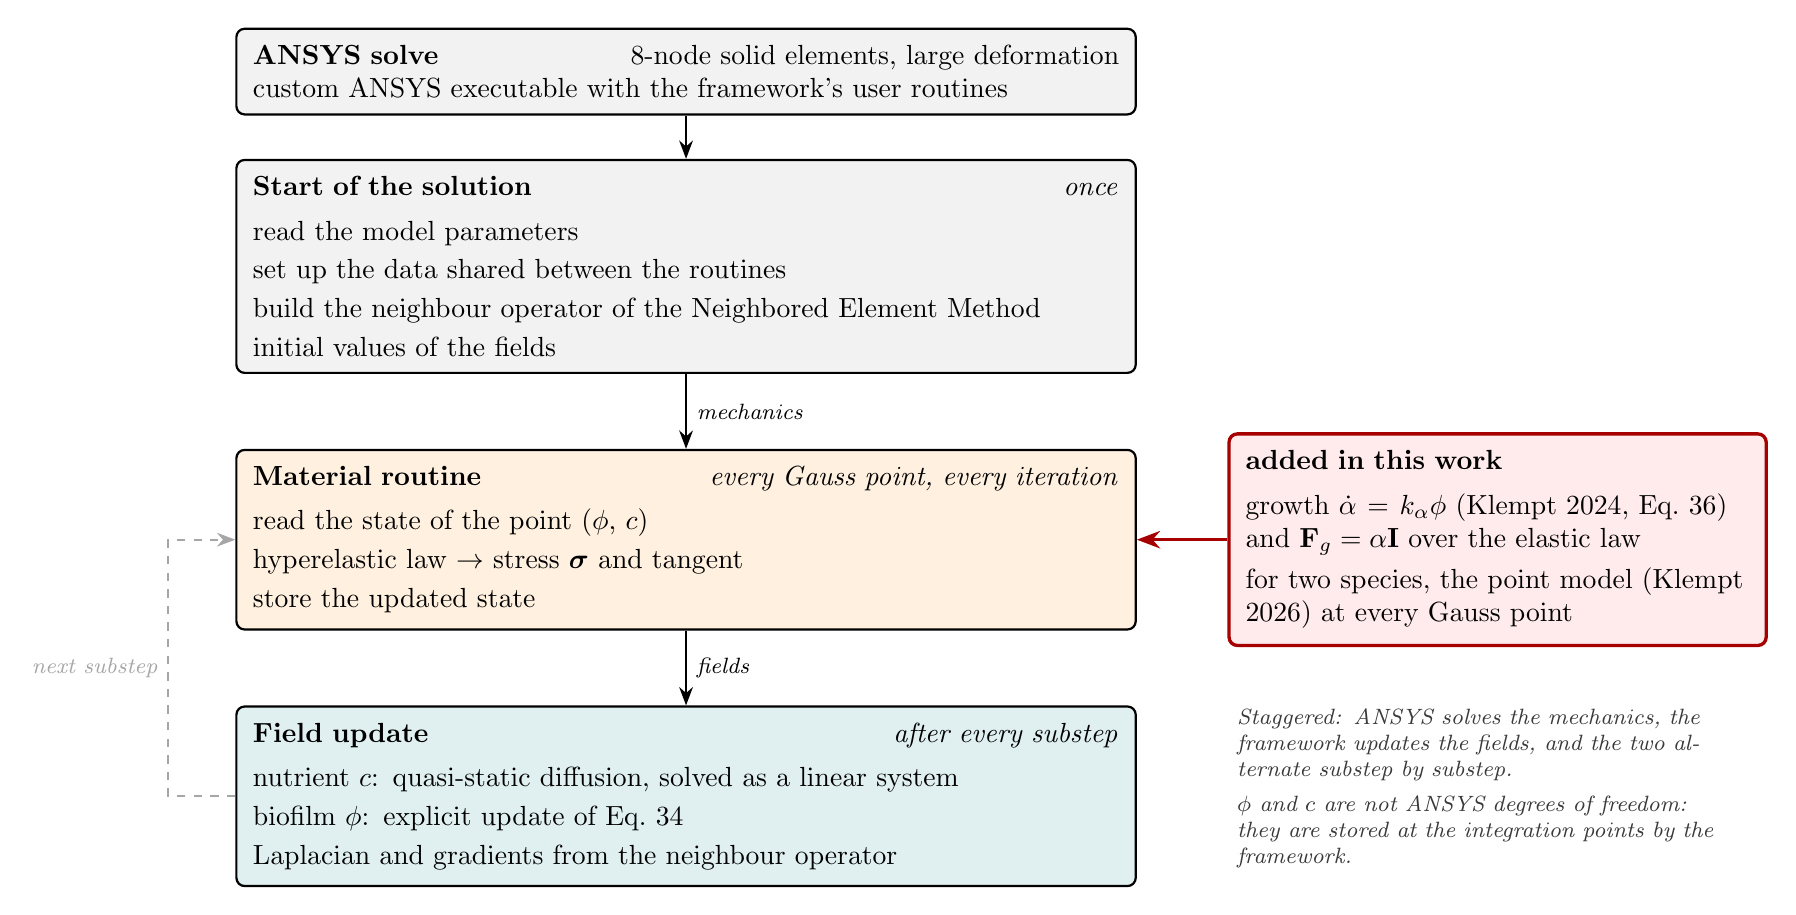
\begin{tikzpicture}[
  every node/.style = {font=\small},
  N/.style    = {draw, rounded corners=3pt, align=left, thick,
                 text width=\olboxwidth, inner sep=6pt},
  Nonce/.style= {N, fill=gray!10},
  Ngp/.style  = {N, fill=orange!12},
  Nfld/.style = {N, fill=teal!12},
  Nours/.style= {draw, rounded corners=3pt, align=left, very thick,
                 draw=red!65!black, fill=red!8, text width=6.4cm, inner sep=6pt},
  ar/.style   = {-Stealth, thick},
  arb/.style  = {-Stealth, thick, dashed, gray!70},
  lbl/.style  = {font=\scriptsize\itshape, fill=white, inner sep=1.5pt, align=center},
  note/.style = {font=\scriptsize\itshape, align=left, text width=6.2cm, gray!45!black},
]

% ── entry ───────────────────────────────────────────────────────────
% Reworded 6 Oct 2026 for the thesis: what each stage does, without the
% framework's internal routine and variable names and without the inherited
% lines that play no part in this work.
\node[Nonce] (top) {%
  \textbf{ANSYS solve} \hfill 8-node solid elements, large deformation\\
  custom ANSYS executable with the framework's user routines};

% ── start of the solution ──────────────────────────────────────────
\node[Nonce, below=0.55cm of top] (beg) {%
  \textbf{Start of the solution} \hfill \textit{once}\\[4pt]
  read the model parameters\\[2pt]
  set up the data shared between the routines\\[2pt]
  build the neighbour operator of the Neighbored Element Method\\[2pt]
  initial values of the fields};
\draw[ar] (top) -- (beg);

% ── the staggered loop ──────────────────────────────────────────────
\node[Ngp, below=0.95cm of beg] (gp) {%
  \textbf{Material routine} \hfill \textit{every Gauss point, every iteration}\\[4pt]
  read the state of the point ($\phi$, $c$)\\[2pt]
  hyperelastic law $\rightarrow$ stress $\bm\sigma$ and tangent\\[2pt]
  store the updated state};
\draw[ar] (beg) -- node[lbl,right,xshift=2pt] {mechanics} (gp);

\node[Nfld, below=0.95cm of gp] (fld) {%
  \textbf{Field update} \hfill \textit{after every substep}\\[4pt]
  nutrient $c$: quasi-static diffusion, solved as a linear system\\[2pt]
  biofilm $\phi$: explicit update of Eq.~34\\[2pt]
  Laplacian and gradients from the neighbour operator};
\draw[ar] (gp) -- node[lbl,right,xshift=2pt] {fields} (fld);

% staggered feedback
\draw[arb] (fld.west) -- ++(-0.85,0) |- node[lbl,pos=0.25,left,xshift=-2pt]
  {next substep} (gp.west);

% ── attachment point of this work ───────────────────────────────────
\node[Nours, right=1.15cm of gp] (ours) {%
  \textbf{added in this work}\\[4pt]
  \small growth $\dot\alpha=k_\alpha\phi$ (Klempt 2024, Eq.~36) and
  $\mathbf F_g=\alpha\mathbf I$ over the elastic law\\[3pt]
  \small for two species, the point model (Klempt 2026) at every Gauss point};
\draw[ar, draw=red!65!black, very thick] (ours) -- (gp);

% ── annotation ──────────────────────────────────────────────────────
\node[note, right=1.15cm of fld, yshift=0.1cm] (n1) {%
  Staggered: ANSYS solves the mechanics, the framework updates the fields,
  and the two alternate substep by substep.\\[3pt]
  $\phi$ and $c$ are not ANSYS degrees of freedom: they are stored at the
  integration points by the framework.};

\end{tikzpicture}

\end{document}
